
\documentclass[12pt,oneside,a4paper,doublespacing]{article} % for submission
%\documentclass[12pt,oneside,a4paper]{article} % for sharing
\usepackage{apacite}
\usepackage{appendix}
\usepackage{amsmath}
\usepackage{amsthm}

\usepackage{amssymb} % for approx greater than
\usepackage{caption}
\usepackage{placeins} % for \FloatBarrier
\usepackage{graphicx}
\usepackage{subcaption}
\usepackage{longtable}
\usepackage{setspace}
\usepackage{booktabs}
\usepackage{tabularx}
\usepackage{xcolor,colortbl}
\usepackage{chngpage}
\usepackage{natbib}
\bibpunct{(}{)}{,}{a}{}{;} 
\usepackage{url}
\usepackage{nth}
\usepackage{authblk}
\usepackage[most]{tcolorbox}
\usepackage[normalem]{ulem}
\usepackage{amsfonts}
% columns for longtable
\newcolumntype{C}[1]{>{\centering\let\newline\\\arraybackslash\hspace{0pt}}m{#1}}
\newcolumntype{L}[1]{>{\raggedright\let\newline\\\arraybackslash\hspace{0pt}}m{#1}}
\usepackage{arydshln} % Dashed lines in matrices

\usepackage[margin=1in]{geometry}
%\doublespacing % for review

% places figures and tables at end.
\usepackage[nolists,nomarkers]{endfloat}
\DeclareDelayedFloatFlavor{longtable}{table}

%%%%%%%%%%%%%%%%%%%%%%%%%%%%%%%%%%%%%%%%%%%%%%%%%%%%%%%%%%%%%%%%%%%%%%%%%%%%%%
% for section 4 math environments
\theoremstyle{definition}
\newtheorem{definition}{Definition}[section]
\newtheorem{theorem}{Theorem}[section]
\newtheorem{proposition}{Proposition}[section]
\newtheorem{corollary}{Corollary}[proposition]
\newtheorem{remark}{Remark}[section]

%%%%%%%%%%%%%%%%%%%%%%%%%%%%%%%%%%%%%%%%%%%%%%%%%%%%%%%%%%%%%%%%%%%%%%%%%%%%%%

\newcommand\ackn[1]{%
  \begingroup
  \renewcommand\thefootnote{}\footnote{#1}%
  \addtocounter{footnote}{-1}%
  \endgroup
}

%%%%%%%%%%%%%%%%%%%%%%%%%%%%%%%%%%%%%%%%%%%%%%%%%%%%%%%
% functions to read in table elements for timelines and graphs table in sec 4
\newcommand{\Ed}[1]{\includegraphics[scale=.45]{{edgep#1}.pdf}}
\newcommand{\Tl}[1]{\includegraphics[scale=.45]{{linep#1}.pdf}}
\newcommand{\St}[1]{\includegraphics[scale=.45]{{starp#1}.pdf}}

% Affiliations in small font size
\renewcommand\Affilfont{\small}


\defcitealias{HMD}{HMD 2016}

% junk for longtable caption
\AtBeginEnvironment{longtable}{\linespread{1}\selectfont}
\setlength{\LTcapwidth}{\linewidth}

% sort van Raalte properly
% #1: sorting key, #2: prefix for citation, #3: prefix for bibliography
\DeclareRobustCommand{\VAN}[3]{#2} % set up for citation

%%%%%%%%%%%%%%%%%%%%%%%%%%%%%%%
\begin{document}

\title{A unified framework of demographic time \\ Figures and Tables only}
\author{[Authors]}

% Table 1
\begin{table}[ht!]
\centering
\caption{~}
\label{tab:sixdefs}
\begin{adjustwidth}{0em}{0em}
\begin{tabular}{lll}
\hline 
\textbf{Time measure}	& \textbf{Demographic definition}	& \textbf{Event history definition}	\\ \hline 
A - chronological age 	& time since birth 			& time since start of exposure 		\\
P - period 		        & calendar time 			& calendar time				\\
C - birth cohort 	    & calendar time of birth 	& calendar time of exposure
start
\\
T - thanatological age 	& time until death 			& time until event			\\
D - death cohort	    & calendar time of death	& calendar time of event		\\
L - lifespan		    & duration of life			& duration of exposure			\\ \hline
\end{tabular}
\end{adjustwidth}
\end{table}

% Table 2: (includes images)
\begin{longtable}{m{0.15\textwidth}L{0.5\textwidth}C{0.2\textwidth}}
\caption{~}
  %\caption{All dyadic juxtapositions of the six measures of demographic time.}
  \label{tab:dyads}\\
 
  \toprule
  \multicolumn{3}{m{0.9\textwidth}}{\footnotesize \emph{Note:} The temporal
  planes are named after the two given time scales. The derived scale is appended in parentheses. Contrary to mathematical convention we name the ordinate scale first and the abscissa scale second. This is to be consistent with the established APC and ACP terms.} \\
   \midrule
  %%%%%%%%%%%%%%%%%%%%%%%%%%%%%%%%%%%%%%%%%%%%%%%%%%%%%%%%%%%%%%%%%%%%%%%%%%%%%
  \multicolumn{3}{c}{\textsc{Variants of APC}} \\
  \midrule
  %%%% APc
  $$\begin{aligned}
    &\text{AP(C)} \\
    &\text{C = P -- A}
  \end{aligned}$$ &
  The AP(C) temporal plane constitutes the classical Lexis diagram. &
  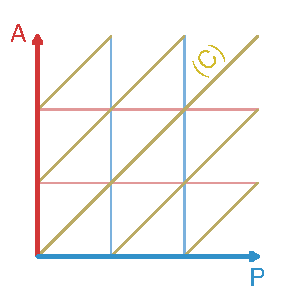
\includegraphics[scale=.5]{AP_rt.pdf}
  \\
  %%%% ACp
  $$\begin{aligned}
    &\text{AC(P)} \\
    &\text{P = C + A}
  \end{aligned}$$ &
  The AC(P) temporal plane is equivalent to the Lexis diagram except birth
  cohort is given and period is derived rather than the other way around. &
  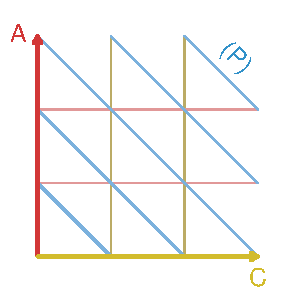
\includegraphics[scale=.5]{AC_rt.pdf} 
   \\
  %%%% CPa
  $$\begin{aligned}
    &\text{CP(A)} \\
    &\text{A = P -- C}
  \end{aligned}$$ &
  The CP(A) temporal plane is equivalent to the Lexis diagram except birth
  cohorts are given and age is derived rather than the other way around. &
  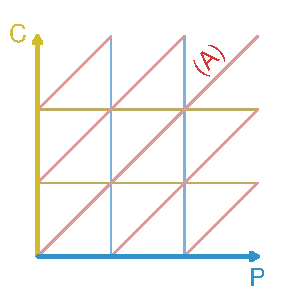
\includegraphics[scale=.5]{CP_rt.pdf}  
  \\
  \midrule
  %%%%%%%%%%%%%%%%%%%%%%%%%%%%%%%%%%%%%%%%%%%%%%%%%%%%%%%%%%%%%%%%%%%%%%%%%%%%%
  \multicolumn{3}{c}{\textsc{Variants of TPD}} \\
  \midrule
  %%%% TPd
  $$\begin{aligned}
    &\text{TP(D)} \\
    &\text{D = P + T}
  \end{aligned}$$ &
  Helen had 30 years of life left (T) in 1971 (P) and therefore belonged to the 2001 death cohort (D) &
  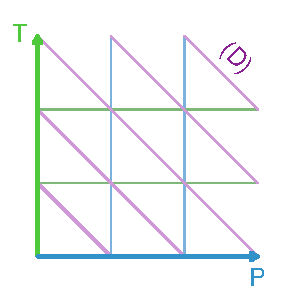
\includegraphics[scale=.5]{TP_rt.pdf}  
   \\
  %%%% PDt
  $$\begin{aligned}
    &\text{PD(T)} \\
    &\text{T = D -- P}
  \end{aligned}$$ &
  Mindel died in 1973 (D). In 1953 (P) she had 20 years left to live (T). &
  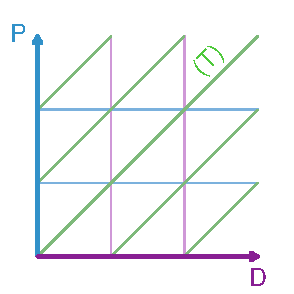
\includegraphics[scale=.5]{PD_rt.pdf} 
   \\
  %%%% TDp
  $$\begin{aligned}
    &\text{TD(P)} \\
    &\text{P = D -- T}
  \end{aligned}$$ &
  Irene died in 1974 (D). When she had 30 remaining years of life (T) the year must have been 1944 (P). &
  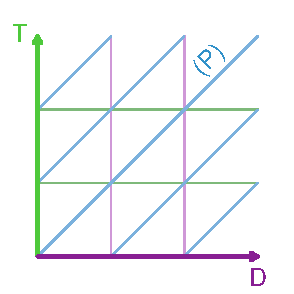
\includegraphics[scale=.5]{TD_rt.pdf}   
  \\
  \midrule
  %%%%%%%%%%%%%%%%%%%%%%%%%%%%%%%%%%%%%%%%%%%%%%%%%%%%%%%%%%%%%%%%%%%%%%%%%%%%%
  \multicolumn{3}{c}{\textsc{Variants of TAL}} \\
  \midrule
  %%%% TAl
  $$\begin{aligned}
    &\text{TA(L)} \\
    &\text{L = T + A}
  \end{aligned}$$ &
  The time already lived and the time still left sum up to the total lifespan. &
  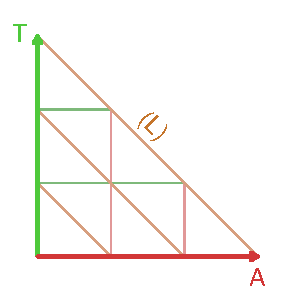
\includegraphics[scale=.5]{TA_rt.pdf}   
  \\
  %%%% TLa
  $$\begin{aligned}
    &\text{TL(A)} \\
    &\text{A = L -- T}
  \end{aligned}$$ &
  Helen lived to the age of 86 (L). When she had 20 years left (T) she must have been 66 (A). &
  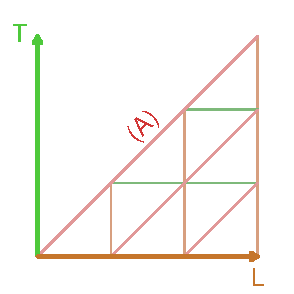
\includegraphics[scale=.5]{TL_rt.pdf}   
 \\
  %%%% ALt
  $$\begin{aligned}
    &\text{AL(T)} \\
    &\text{T = A -- L}
  \end{aligned}$$ &
  Tim is 34 years old (A) and will live to the age of 96 (L), leaving him 62 years (T) to settle affairs. &
  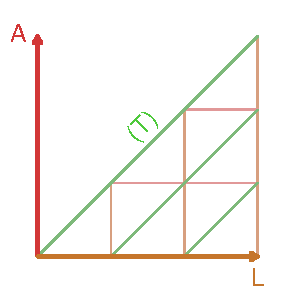
\includegraphics[scale=.5]{AL_rt.pdf} 
  \\
  \midrule
  %%%%%%%%%%%%%%%%%%%%%%%%%%%%%%%%%%%%%%%%%%%%%%%%%%%%%%%%%%%%%%%%%%%%%%%%%%%%%
  \multicolumn{3}{c}{\textsc{Variants of LCD}} \\
  \midrule
  %%%% LCd
  $$\begin{aligned}
    &\text{LC(D)} \\
    &\text{D = C + L}
  \end{aligned}$$ &
  \`{A}ngels was born in 1940 (C) and she lived to be 64 (L), implying an
  untimely death in 2004 (D) &
  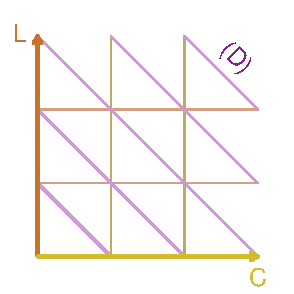
\includegraphics[scale=.5]{LC_rt.pdf}   
  \\
  %%%% CDl
  $$\begin{aligned}
    &\text{CD(L)} \\
    &\text{L = D -- C}
  \end{aligned}$$ &
  Pascal was born in 1893 (C) and died in 1964 (D), implying a lifespan of 71 (L), or so. &
  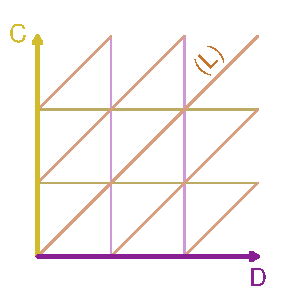
\includegraphics[scale=.5]{CD_rt.pdf} 
  \\
  %%%% LDc
  $$\begin{aligned}
    &\text{LD(C)} \\
    &\text{C = D -- L}
  \end{aligned}$$ &
  Margaret died in Dec., 1995 (D) with a completed lifespan of 96 (L), putting her birth year in 1900 (C). &
  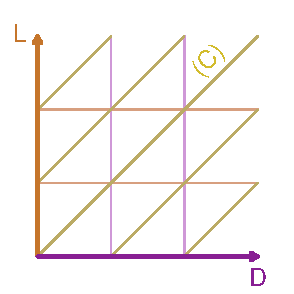
\includegraphics[scale=.5]{LD_rt.pdf}  
  \\
  \midrule
  %%%%%%%%%%%%%%%%%%%%%%%%%%%%%%%%%%%%%%%%%%%%%%%%%%%%%%%%%%%%%%%%%%%%%%%%%%%%%
  \multicolumn{3}{c}{\textsc{The Uninformative Dyads}} \\
  \midrule
  %%%% LP
  LP(-) &
  The LP plane is \emph{non-informative}. No additional measures can be derived knowing just lifespan and period. &
  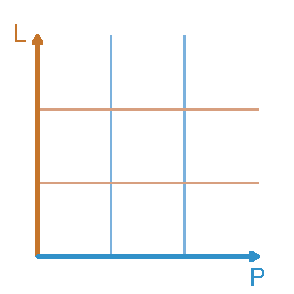
\includegraphics[scale=.5]{LP_rt.pdf} 
  \\
  %%%% CT
  CT(-) &
  The CT plane is \emph{non-informative}. No additional measures can be derived
  knowing just birth cohort and thanatological age. &
  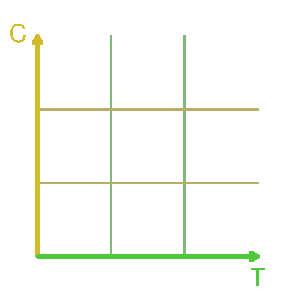
\includegraphics[scale=.5]{CT_rt.pdf} \\
  %%%% AD
  AD(-) &
  The AD plane is \emph{non-informative}. No additional measures can be derived
  knowing just death cohort and age. &
  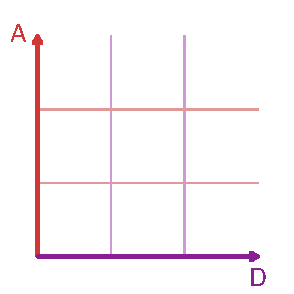
\includegraphics[scale=.5]{AD_rt.pdf} 
\\
  \bottomrule
\end{longtable}

\newcolumntype{S}{ >{\centering\arraybackslash} m{2cm} }
\newcolumntype{D}{ >{\centering\arraybackslash} m{5.4cm} }
\newcolumntype{E}{ >{\centering\arraybackslash} m{3.7cm} }

% Table 3  (includes images)
\begin{table}[ht]
\centering
\caption{~}
%\caption{Event-duration timeline and graph for two, three, and four event
% sequences.}
%\label{tab:timelines}
\makebox[\linewidth][c]{
\begin{tabular}{S D E}
nr. events  & timeline & graph \\
& &\\
  $n = 2 $ & \Tl{2} & \Ed{2} \\
  $n = 3 $ & \Tl{3} & \Ed{3} \\
  $n = 4 $ & \Tl{4} & \Ed{4}
\end{tabular}
}
\end{table}

% Figure 1
\begin{figure}[h!] 
\caption{~}
%\caption{An APC diagram with six lifelines.}
%\label{fig:APC}
%\centering
%\vspace{-5em}
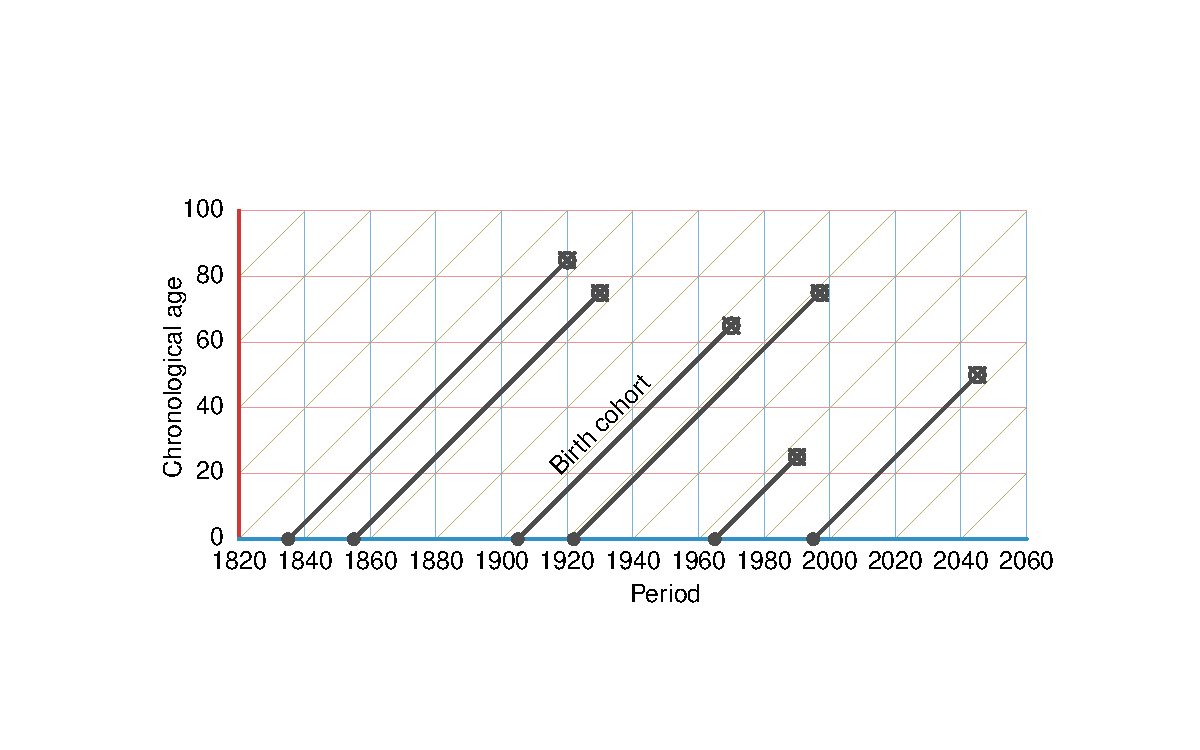
\includegraphics[scale=0.8]{APCrt.pdf}
\end{figure}

% Figure 2
\begin{figure}[h!] 
\caption{~}
%\caption{A TPD diagram with six lifelines.}
%\label{fig:TPD}
%\centering
%\vspace{-5em}
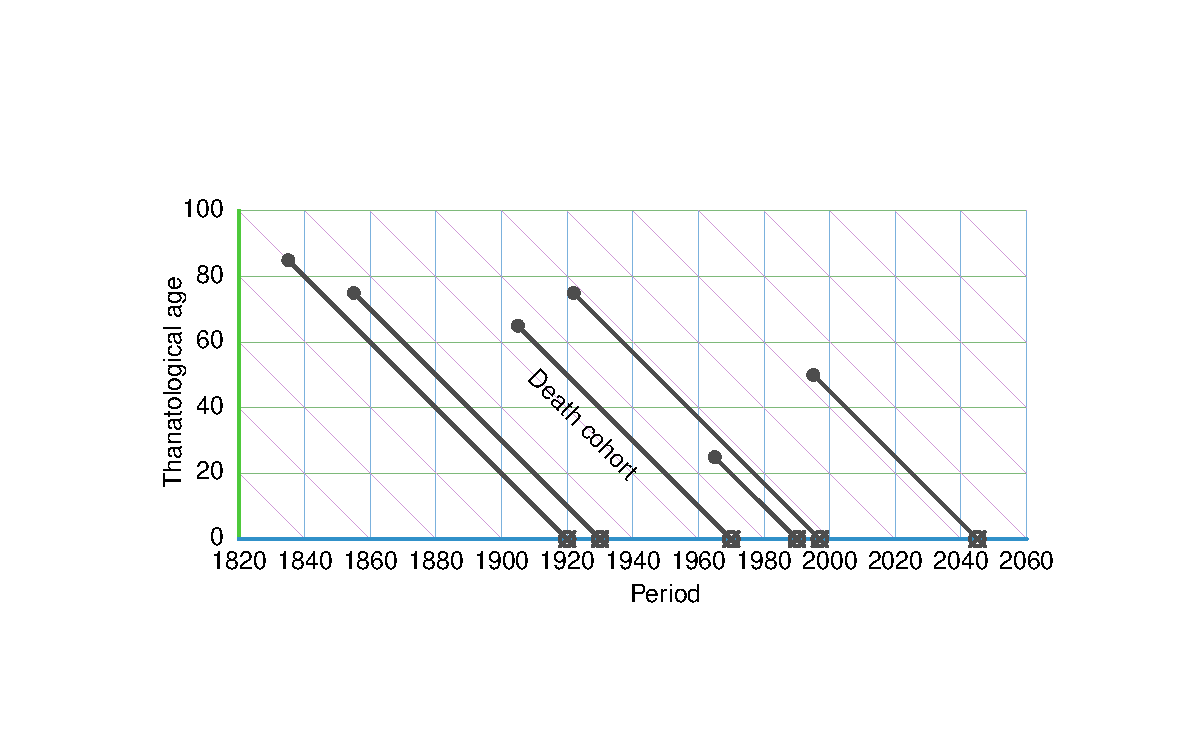
\includegraphics[scale=0.8]{TPDrt.pdf}
\end{figure} 

% Figure 3
\begin{figure}[h!] 
\caption{~}
%\caption{A TAL diagram with six lifelines. Since two of the six lifelines are of equal length (75), they are
%overlapped in this figure and appear to be five.}
%\label{fig:TAL}
\centering
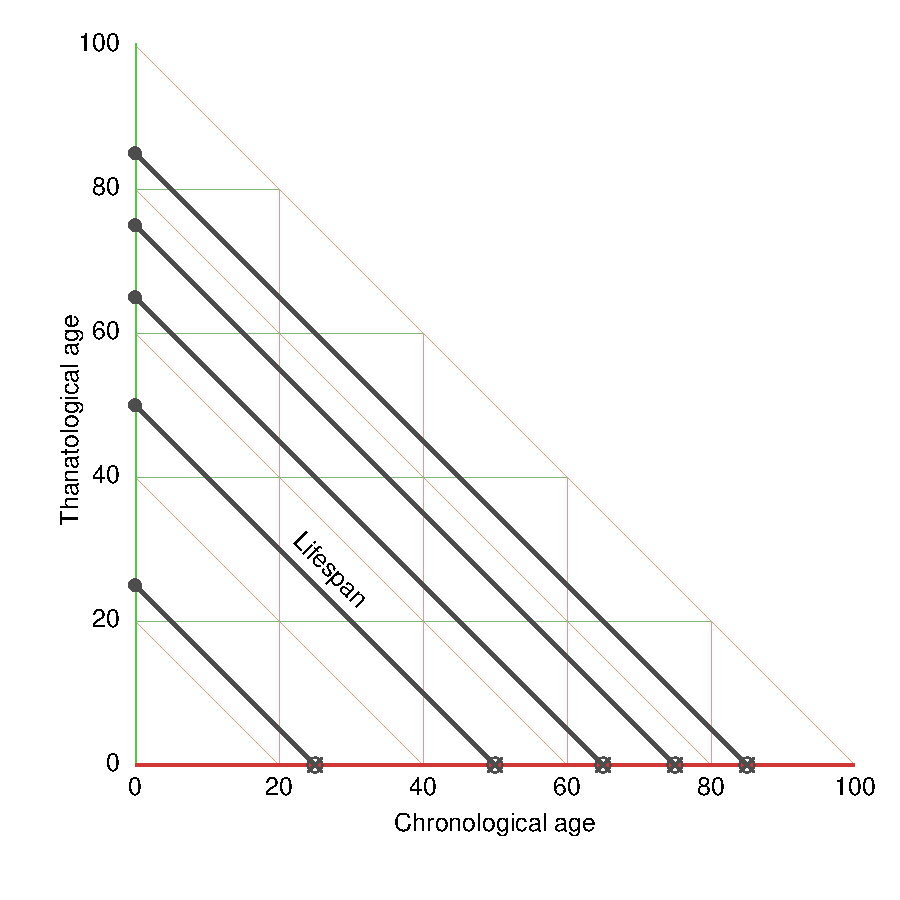
\includegraphics[scale=0.7]{TALrt.pdf}
\end{figure} 

% Figure 4
\begin{figure}[h!] 
\caption{~}
%\caption{An LCD diagram with six lifelines. Since the LCD plane is orthogonal
%to the life course, lifelines are depicted as points.}
%\label{fig:LCD}
%\centering
%\vspace{-5em}
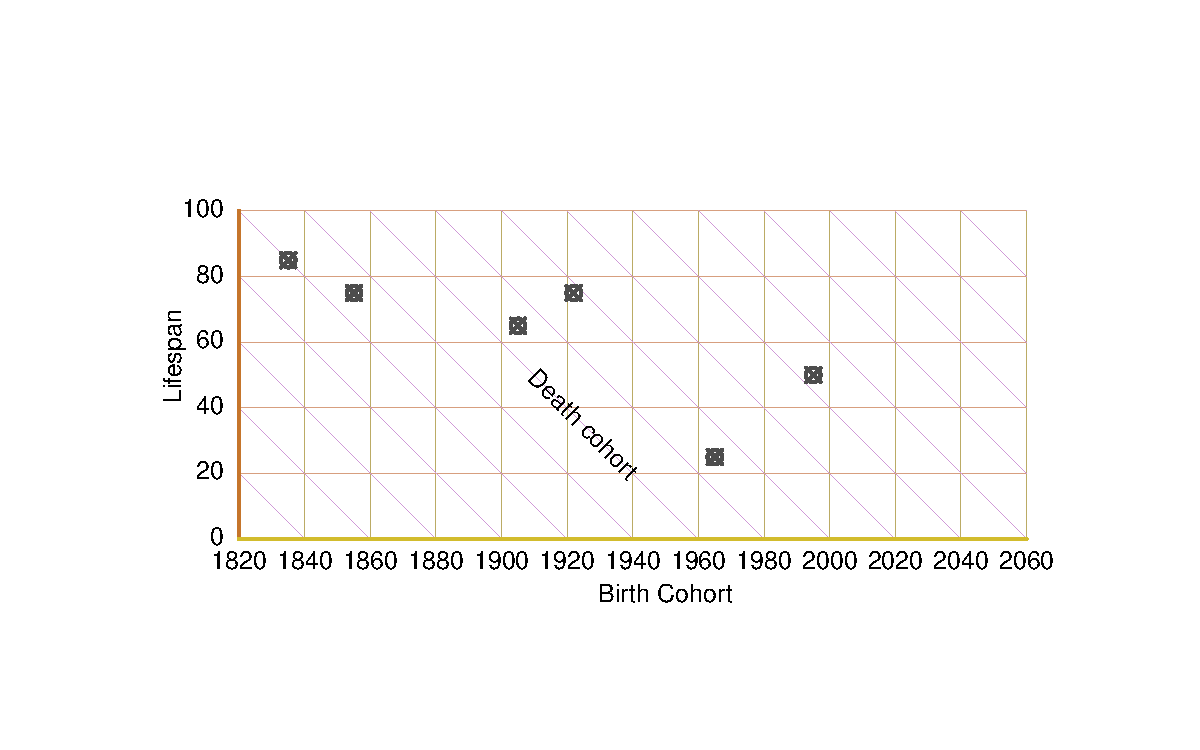
\includegraphics[scale=0.8]{LCDrt.pdf}
\end{figure} 

% Figure 5
\begin{figure}[h!]
\centering
\caption{~}
%\caption{Tetrahedral graph of demographic time hexad identity, with edges
%labelled by the six time indices.}
%\label{fig:tet}
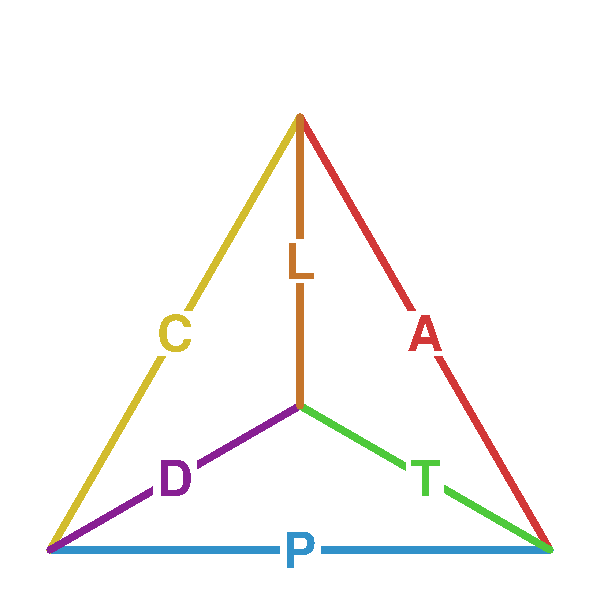
\includegraphics[width=4in]{TetraHedronEdgesOnly.pdf}%
\end{figure}

% Figure 6
\begin{figure}[!h]
\centering
\caption{~}
%\caption[cap]{Diagram of the hexad identity, showing a sequence of TAL
%planes intersecting with a single APC plane at the base.}
%\label{fig:apctTAL}
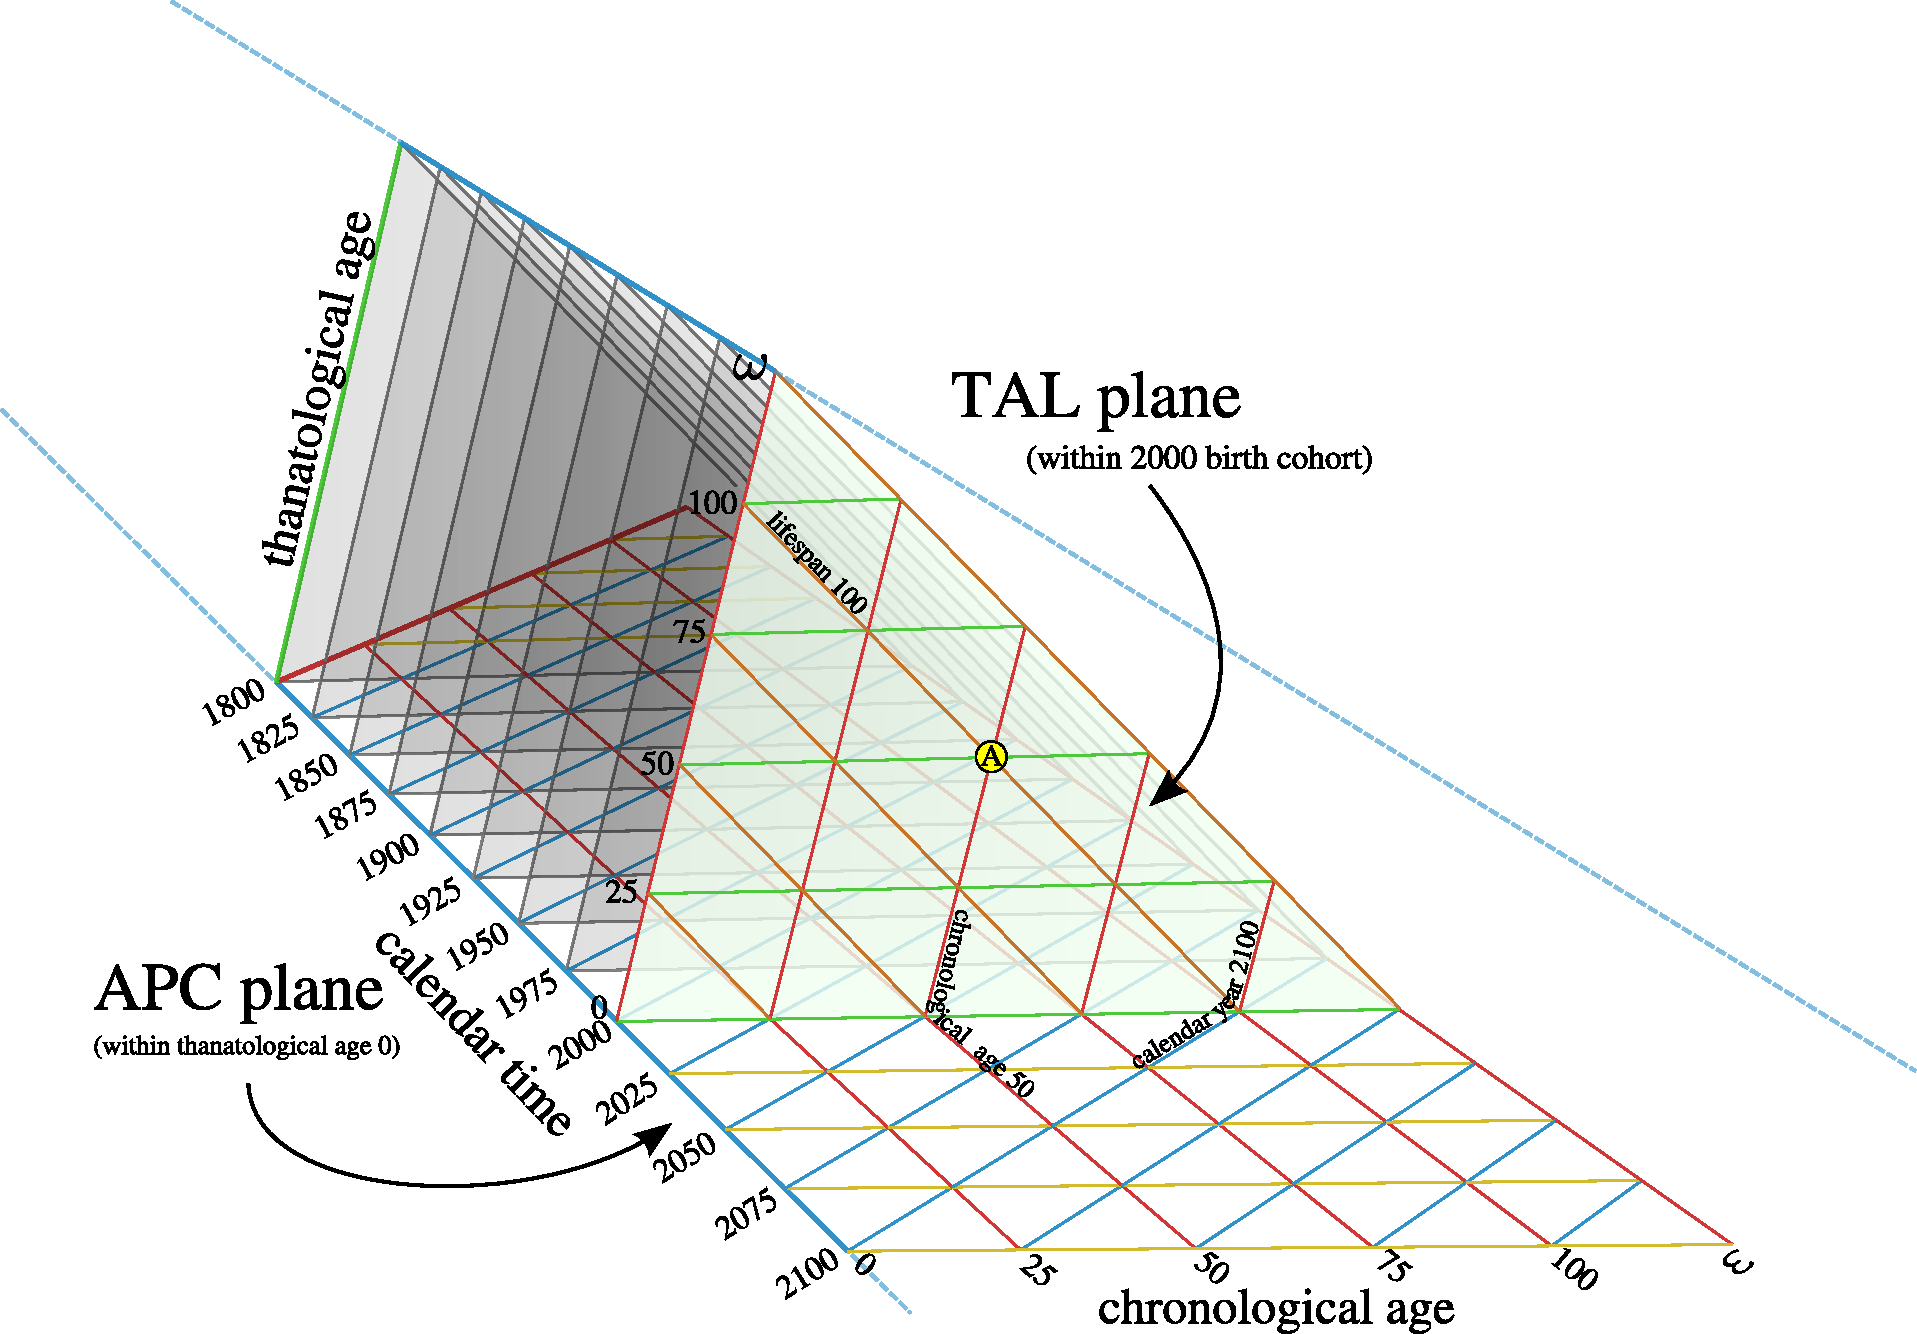
\includegraphics[scale=.5]{TALisomarkedup2.pdf}
\end{figure}

% Figure 7 (panel)
\begin{figure}[h!] 
%\caption{Prevalence of males self-reporting poor health by chronological and
%thanatological age, by quinquennial birth cohorts, 1905--1925 (Sources: \citealt{HRSumich, HRS})}
%\label{fig:poorsrh}
\centering
\caption{~}
\vspace{-1em}
\begin{subfigure}{.46\textwidth}
\centering
%\caption{1905}
%\vspace{-1em}
%\label{fig:srh1905}
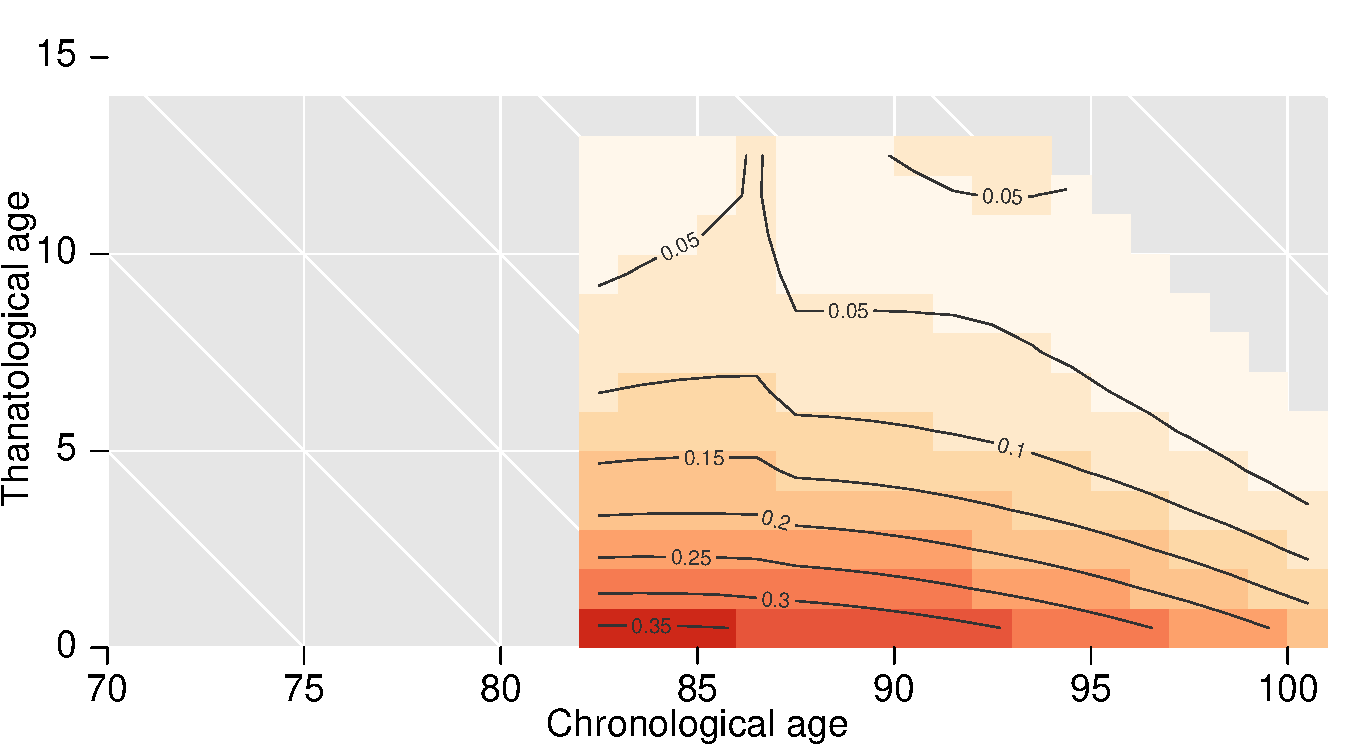
\includegraphics[scale=0.32]{srhpoor1905.pdf}
\end{subfigure}
~
\begin{subfigure}{.46\textwidth}
\centering
%\caption{1910}
%\vspace{-1em}
%\label{fig:srh1910}
%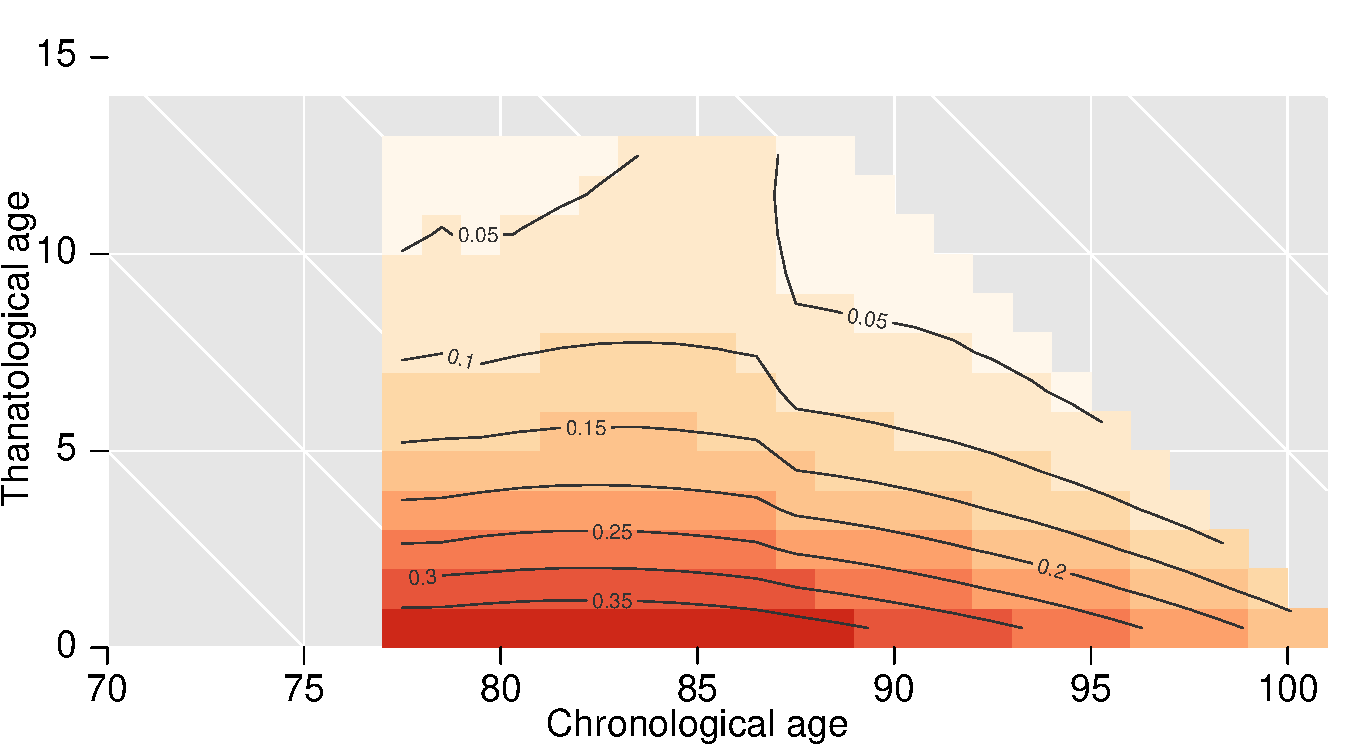
\includegraphics[scale=0.32]{srhpoor1910.pdf}
\end{subfigure}

\begin{subfigure}{.46\textwidth}
\centering
\caption{~}
%\caption{1915}
%\vspace{-1em}
%\label{fig:srh1915}
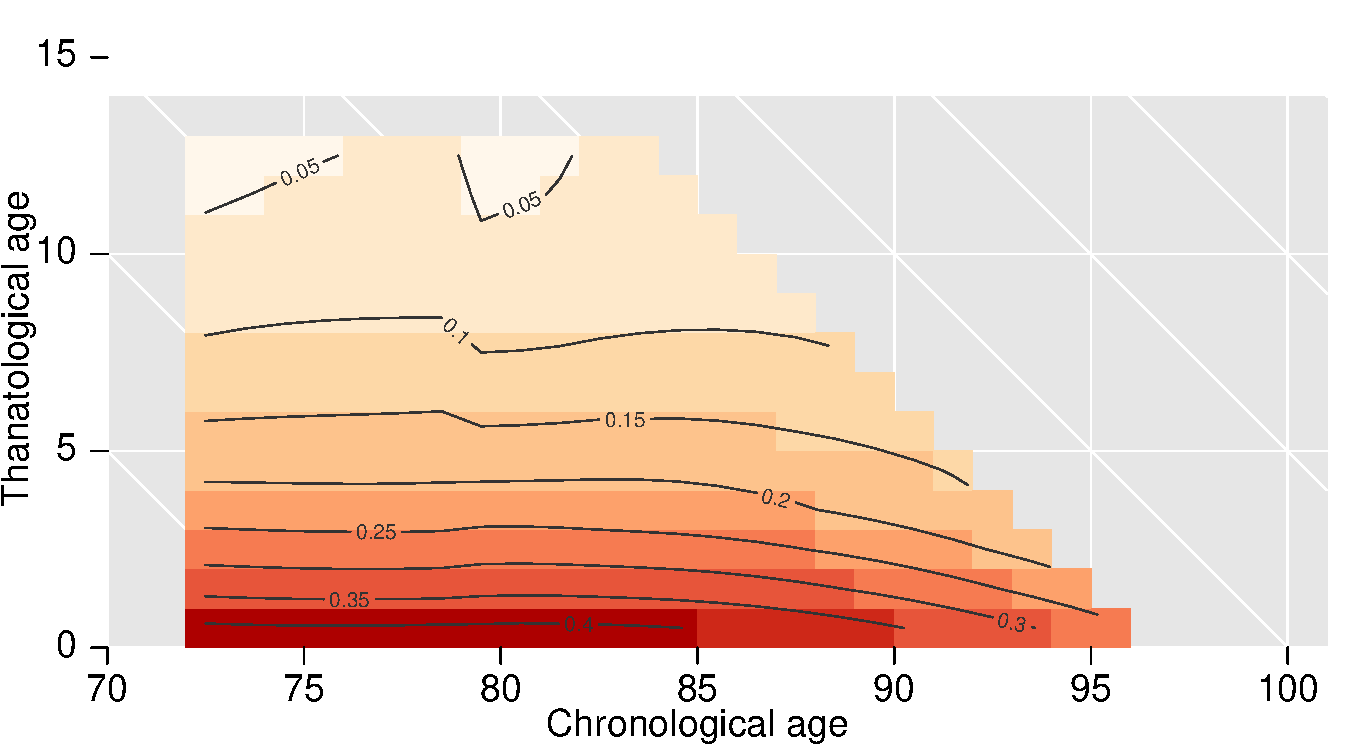
\includegraphics[scale=0.32]{srhpoor1915.pdf}
\end{subfigure}
~
\begin{subfigure}{.46\textwidth}
\centering
\caption{~}
%\caption{1920}
%\vspace{-1em}
%\label{fig:srh1920}
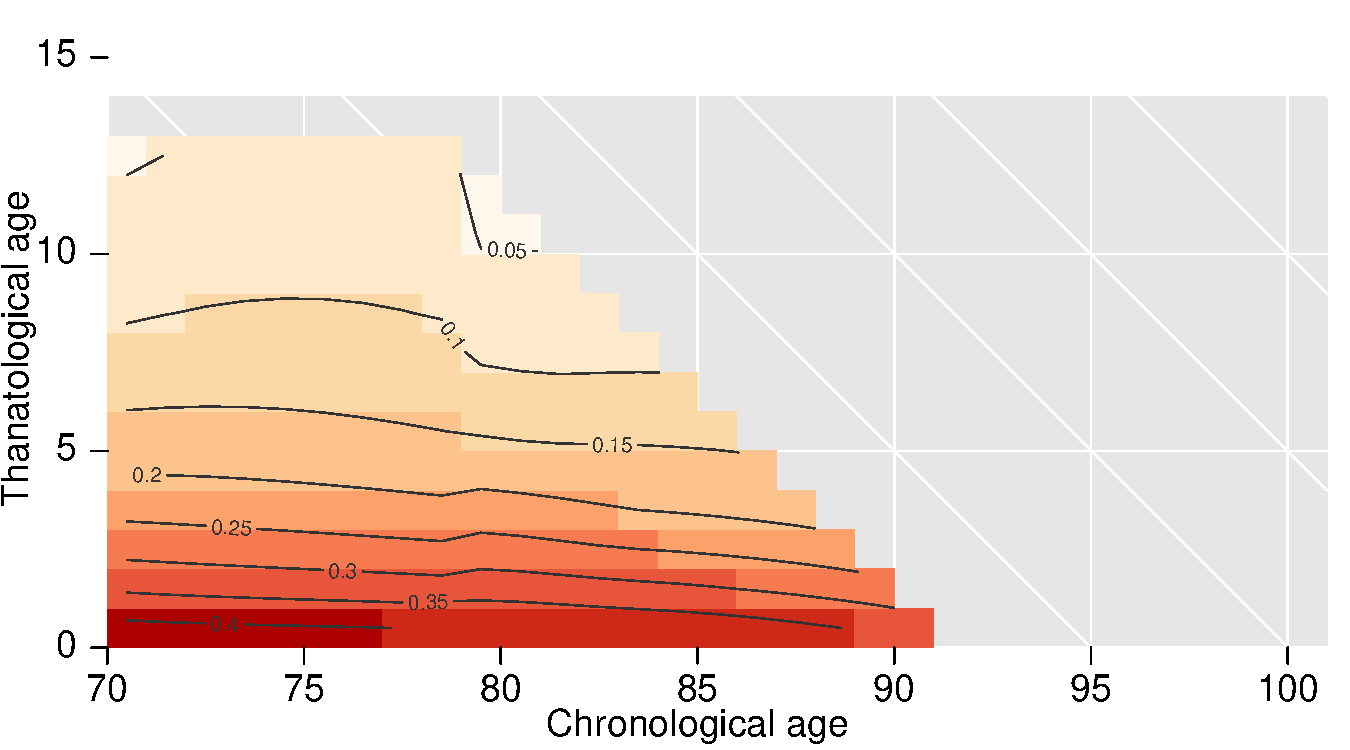
\includegraphics[scale=0.32]{srhpoor1920.pdf}
\end{subfigure}

\begin{subfigure}{.46\textwidth}
\centering
\caption{~}
%\caption{1925}
%\vspace{-1em}
%\label{fig:srh1925}
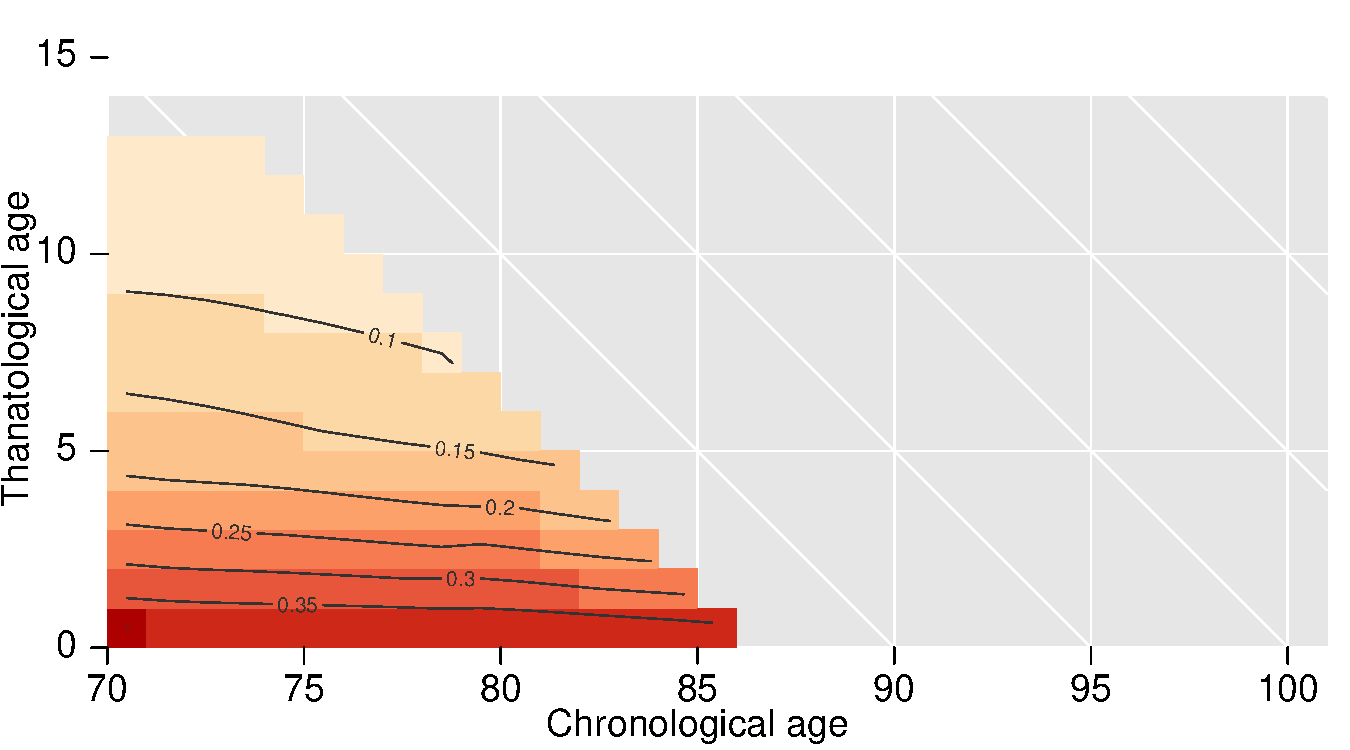
\includegraphics[scale=0.32]{srhpoor1925.pdf}
\end{subfigure}
~
\begin{subfigure}{.46\textwidth}
\centering
\caption{~}
%\caption*{~}
%\vspace{-1em}
%\label{fig:srhlegend}
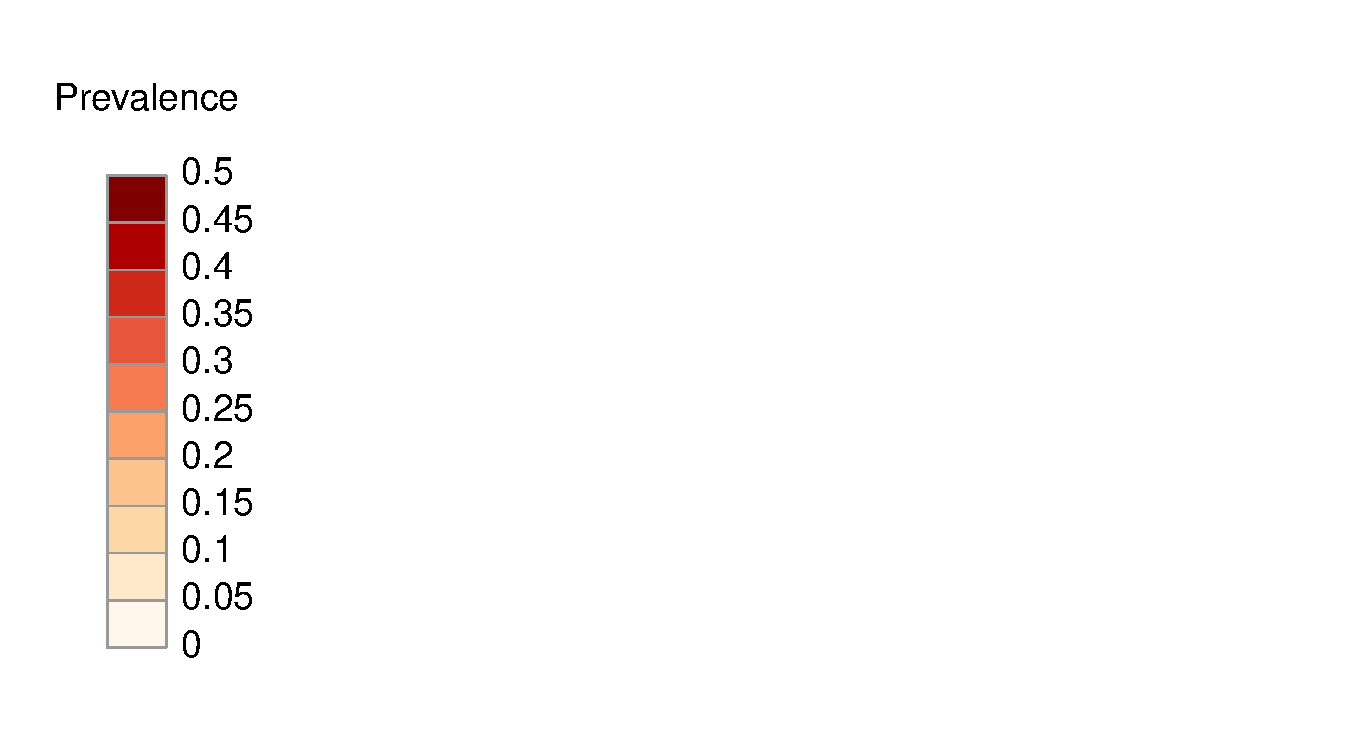
\includegraphics[scale=0.32]{Legend.pdf}
\end{subfigure}
\end{figure} 
\end{document}